\section{Метод конечных разностей для решения одномерного нестационарного уравнения диффузии}
\subsection{Коэффициент диффузии не зависит от концентрации}
Одномерное нестационарное уравнение диффузии, соответствующее второму закону Фика имеет вид:
\begin{equation}\label{eq:difft}
	\frac{\delta}{\delta t} C = D\frac{\delta^{2}}{\delta x^2} C;
\end{equation}

Аппроксимация первой производной по времени в момент времени $t_{i}$ концентрации $C_{j}(t_{i}) = C^{i}_{j}$ в точке $j$:
\begin{equation}\label{eq:diffdt1}
	\frac{\delta}{\delta t} C^{i}_{j} = \frac{C^{i+1}_{j} - C^{i}_{j}}{\Delta t};
\end{equation}

Аппроксимация первой производной по координате в момент времени $t_{i}$ концентрации $C_{j}(t_{i}) = C^{i}_{j}$ в точке $j$:
\begin{equation}\label{eq:diffdx1}
	J^{i}_{j} = \frac{\delta}{\delta x} C^{i}_{j} = \frac{C^{i}_{j+1} - C^{i}_{j}}{\Delta x};
\end{equation}

Аппроксимация второй производной по координате в момент времени $t_{i}$ концентрации $C_{j}(t_{i}) = C^{i}_{j}$ в точке $j$:
\begin{equation*}
	\frac{\delta^{2}}{\delta x^{2}} C^{i}_{j} = \frac{\delta}{\delta x}\bigg[ \frac{C^{i}_{j+1} - C^{i}_{j}}{\Delta x} \bigg] = \frac{ \frac{C^{i}_{j+1} - C^{i}_{j}}{\Delta x} - \frac{C^{i}_{j} - C^{i}_{j-1}}{\Delta x}}{\Delta x} = 
\end{equation*}
\begin{equation}\label{eq:diffdx2}
	= \frac{C^{i}_{j+1} - 2C^{i}_{j} + C^{i}_{j-1}}{\Delta x^2};
\end{equation}

Подставляя в (\ref{eq:difft}) аппроксимацию производных (\ref{eq:diffdt1}), (\ref{eq:diffdx2}), получим связь $C^{i+1}_{j}$ с $C^{i}_{j}$, т.е. изменение концентрации через $\Delta t$:

\begin{equation}\label{eq:diffFD}
	C^{i+1}_{j} = \lambda C^{i}_{j-1} + (1 - 2\lambda)C^{i}_{j} + \lambda C^{i}_{j+1},
\end{equation}
где $\lambda = \frac{D\Delta t}{\Delta x^2}$~---  связь коэффициента диффузии и шагов по сетке времени и координаты.

Уравнение (\ref{eq:diffFD}) справедливо для всех не крайних точек конечно разностной схемы, при коэффициенте диффузии не зависящем от концентрации.

Выделим два граничных приближения для концентрации:
\begin{enumerate}
	\item <<Закрытая система>> ~--- концентрация на границе не изменяется ($J_{0}^{i} = 0$, $J_{N+1}^{i} = 0$), см. рис.\ref{fig:CD};
	\item <<Открытая система>> ~--- поток частиц подходящий к границе равен потоку уходящих частиц ($J_{0}^{i} = J_{1}^{i}$, $J_{N}^{i} = J_{N+1}^{i}$), см. рис.\ref{fig:OD}.
\end{enumerate}

\begin{figure}
	\centering
	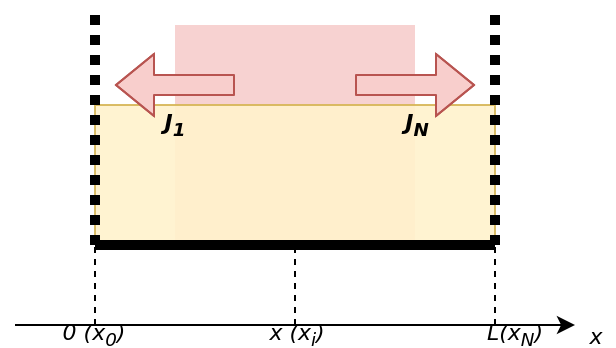
\includegraphics[width=0.9\linewidth]{assets/CD}
	\caption{"Закрытая" система диффузии}
	\label{fig:CD}
\end{figure}

\begin{figure}
	\centering
	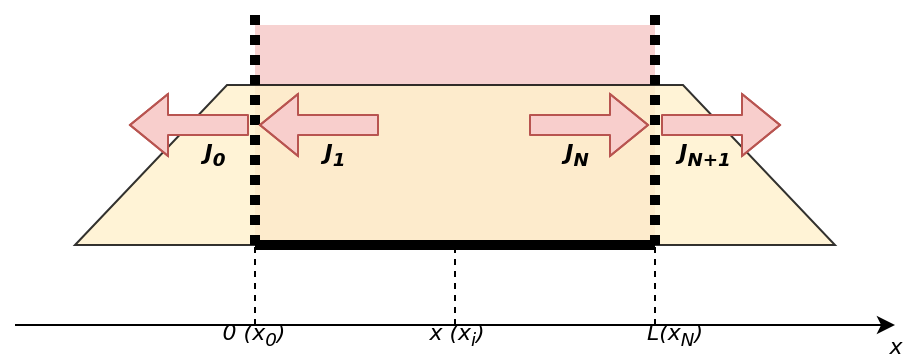
\includegraphics[width=0.9\linewidth]{assets/OD}
	\label{fig:OD"}
\end{figure}

Для <<закрытой системы>> должно выполняться условие $J_{0}^{i} = 0$, $J_{N+1}^{i} = 0$. Рассмотрим (\ref{eq:diffdx1}), (\ref{eq:diffFD}) для точки $j = 1$:
\begin{gather*}
 	J^{i}_{0} = \frac{C^{i}_{1} - C^{i}_{0}}{\Delta x} = 0 \Rightarrow C_{0}^{i} = C_{1}^{i};\\
	C^{i+1}_{1} = \lambda C^{i}_{0} + (1 - 2\lambda)C^{i}_{1} + \lambda C^{i}_{2} = \lambda C^{i}_{1} + (1 - 2\lambda)C^{i}_{1} + \lambda C^{i}_{2} = \\
	= (1 - \lambda)C^{i}_{1} + \lambda C^{i}_{2} = C^{i+1}_{1};
\end{gather*}
Рассматривая точки $N-1$, $N$, $N+1$ аналогичным образом получим:
\begin{equation}
	\begin{cases}
		C^{i+1}_{1} = (1 - \lambda)C^{i}_{1} + \lambda C^{i}_{2};\\
		C^{i+1}_{j} = \lambda C^{i}_{j-1} + (1 - 2\lambda)C^{i}_{j} + \lambda C^{i}_{j+1},\,j \in [2,\,\dots,\,N-1];\\
		C^{i+1}_{N} = (1 - \lambda)C^{i}_{N} + \lambda C^{i}_{N-1};\\
		\lambda = D\frac{\Delta t}{\Delta x^{2}}.
	\end{cases}
\end{equation}

Для <<открытой>> системы должно выполняться условие $J_{0}^{i} = J_{1}^{i}$, $J_{N}^{i} = J_{N+1}^{i}$. Рассмотрим (\ref{eq:diffdx1}), (\ref{eq:diffdx2}), (\ref{eq:diffFD}) для точки $j = 1$:
\begin{gather*}
 	J^{i}_{0} = J^{i}_{1}\\
	\frac{C^{i+1}_{1} - C^{i}_{1}}{\Delta t} = \frac{J^{i}_{1} - J^{i}_{0}}{\Delta x} = \frac{0}{\Delta x} = 0\Rightarrow\\
	\Rightarrow C^{i+1}_{1} = C^{i}_{1};
\end{gather*}
Рассматривая точки $N-1$, $N$, $N+1$ аналогичным образом получим:
\begin{equation}
	\label{eq:DDiffConst}
	\begin{cases}
		C^{i+1}_{1} = C^{i}_{1};\\
		C^{i+1}_{j} = \lambda C^{i}_{j-1} + (1 - 2\lambda)C^{i}_{j} + \lambda C^{i}_{j+1},\,j \in [2,\,\dots,\,N-1];\\
		C^{i+1}_{N} = C^{i}_{N};\\
		\lambda = D\frac{\Delta t}{\Delta x^{2}}.
	\end{cases}
\end{equation}

\subsection{Коэффициент диффузии зависит от концентрации}

Если коэффициенте диффузии (D) зависит от концентрации, тогда уравнение диффузии принимает вид:

\begin{equation}\label{eq:diffD(x)t}
	\frac{\delta}{\delta t} C = \frac{\delta}{\delta x}D\frac{\delta}{\delta x} C;
\end{equation}

Тогда уравнение конечно-разностной схемы будет~\cite{MethFD}:
\begin{gather}\label{eq:diffD(x)tFD}
	\frac{C_{j}^{i+1} - C_{j}^{i}}{\Delta t} = \frac{ D_{j+1/2}^{i}\frac{C^{i}_{j+1} - C^{i}_{j}}{\Delta x} - D_{j-1/2}^{i}\frac{C^{i}_{j} - C^{i}_{j-1}}{\Delta x} }{\Delta x};\\
	D_{j\pm1/2}^{i} = \frac{D^{i}_{j} + D^{i}_{j\pm1}}{2} = D_{j\pm}^{i}.
\end{gather}

Проводя рассуждения аналогичные предыдущему параграфу получит конечно-разностную схему для открытой схемы:
\begin{equation}
	\begin{cases}
		C^{i+1}_{1} = C^{i}_{1};\\
		C^{i+1}_{j} = \lambda_{-}^{i} C^{i}_{j-1} + (1 - \lambda^{i}_{+} - \lambda^{i}_{-})C^{i}_{j} + \lambda^{i}_{+} C^{i}_{j+1},\,j \in [2,\,\dots,\,N-1];\\
		C^{i+1}_{N} = C^{i}_{N};\\
		\lambda^{i}_{+} = D_{j+}^{i}\frac{\Delta t}{\Delta x^{2}};\\
		\lambda^{i}_{-} = D_{j-}^{i}\frac{\Delta t}{\Delta x^{2}}.
	\end{cases}
\end{equation}
